\documentclass[a4paper]{article}

%use the english line for english reports
\usepackage[english]{babel}
%\usepackage[portuguese]{babel}
\usepackage[utf8]{inputenc}
\usepackage{indentfirst}
\usepackage{enumerate}
\usepackage{graphicx}
\usepackage{verbatim}
\usepackage{url}


\begin{document}

\setlength{\textwidth}{16cm}
\setlength{\textheight}{22cm}

\title{\Huge\textbf{Mbrane}\linebreak\linebreak\linebreak
\Large\textbf{Final Report}\linebreak\linebreak
\linebreak\linebreak

\includegraphics[scale=0.1]{feup-logo.png}\linebreak\linebreak
\linebreak\linebreak
\Large{Logic Programing}\linebreak
}

\author{\textbf{Group Mbrane 4:}\\ Leonardo Fernandes Moura - 201706907@fe.up.pt \\ João Pedro Campos - up201704982@fe.up.pt \\\linebreak\linebreak \\
 \\ Faculdade de Engenharia da Universidade do Porto \\ Rua Roberto Frias, s\/n, 4200-465 Porto, Portugal \linebreak\linebreak\linebreak
\linebreak\linebreak\vspace{1cm}}
\date{November 13, 2019}
\maketitle
\thispagestyle{empty}

%************************************************************************************************
%************************************************************************************************

\newpage

\section*{Summary}

The goal of this project was to program a board game using the prolog language. In our case the game in question is Mbrane, a 
game created by DukeZhou based on Sudoku and strategy games like chess. Section 2 clarifies all the aspects of this game.

\paragraph{}
In terms of programing, the goal of the project was to efficiently implement all the game logic using Prolog.  This means we have to
represent the core mechanics of the game using Prolog. The first step is to find a way to represent the game board that's both 
efficient and relatively simple to program and operate. Then our goal is to make the game playable, continuously updating the state of
the board as both players make their moves. In order to termiate the game and find the winner, we need to detect when the board is in a completed 
state, then we calculate the winner and present it. After the game is playable, the final step is to make it possible to play against the computer 
programing a bot that would be able to play in two difficulty settings. The first one (the easy mode) simply makes random plays, the second 
one calculates the best play it can make at the moment (greedy approach). This means we end up with three different game modes: player versus player,
player versus bot and bot versus bot. 

\paragraph{}
Besides all the game logic, the player needs to interact with the game, so we need to develop a simple text base UI, using
Prolog predicates that are able to interact with the terminal input/output stream. This allows us to read inputs from the
player (or both players) so that we can use them make moves.

\paragraph{}
The prolog distribution used was SicStus Prolog using a Student License.

\newpage

\tableofcontents

%************************************************************************************************
%************************************************************************************************

%*************************************************************************************************
%************************************************************************************************

\newpage

%%%%%%%%%%%%%%%%%%%%%%%%%%
\section{Introduction}
\paragraph{}
This project was developed during the Logic Programing Course in the context of the third year of the Integrated Masters in Informatics 
and Computing Engineering at FEUP. The goal was to implement the logic of a board game in Prolog, in this case \textit{Mbrane}.

\paragraph{}
Here is a short explanation of all the sections in this report:

\begin{itemize}
    \item \textbf{Game presentation:} Clarification of the most relevant aspets of the game, both it's rules and origin.
    \begin{itemize}
        \item \textbf{Origin:} Description the origin of the game, and it was based on the journals of the game
        creator himself.
        \item \textbf{Rules:} Description of all the rules of the game. 
    \end{itemize}
    
    \item \textbf{Game Logic:} Description of the game logic and how it was implememted in Prolog, it focuses
    on the most relevant predicates.
    \begin{itemize}
        \item \textbf{Game state representation:} Description of how all the different states of the game are represented internally in Prolog. 
        \item \textbf{Board viewing:} Description of how we use the internal game state representation to display the game in a relatively user friendly way, using a text interface.
        \item \textbf{List valid plays:} Description of how the we are able to determine if a play is valid or not, and more importantly, how we can find all the plays that can be made in a given moment.
        \item \textbf{Game finalization:} Description of how we are able to detect the game is in a final state in order to determine the winner.
        \item \textbf{Board Evaliation:} Description of how we can evaluate the board, in order to find if a given play is valid or not.
        \item \textbf{Plays of the computer:} Description of the computer choses a move when given a list of possible moves.
    \end{itemize}
\end{itemize}


%%%%%%%%%%%%%%%%%%%%%%%%%%
\pagebreak
\section{Game Presentation}

\subsection{Origin}

\paragraph{}
Mbrane is a fairly recent game. It was created in 2013 by someone who goes by the name of DukeZhou. 
When he was a kid, DukeZhou really liked to play strategy board games, but he didn’t like games where luck was a 
relevant factor, he liked games where the player with superior strategy or the one “who played better” was definitely the winner. 
Games like chess or checkers were all he was into. n 2005 he discovered Sudoku, and even though puzzles were not his favorite type 
of game, he was amazed by the game. The sheer amount of combinations for a 9x9 board is around $6.7*10^21$. That factor combined with 
the all restraints the puzzle imposes made it feel somewhat magical.

\paragraph{}
In May 2013 while he was playing Fallout 3 the rules of Mbrane dropped into his head all at once. He immediately called a friend whom
he used to play chess with and they spent hours playing and discovering the game, getting more and more fascinated with it as time went by.

\paragraph{}
The full story, taken from the journals of DukeZhou can be read in the following address: 
http://mbranegame.com/origin-of-mbrane \cite{Origin}.

\subsection{Rules}
The following rules are the official rules for Mbrane, in their integral redaction.
Mbrane is divided in two distinct phases: the placement phase and the resolution phase

\subsubsection{Placement phase}
\begin{itemize}
    \item Players take turns placing numbers in an empty Sudoku. These are bids for territories. 
\end{itemize}
\begin{center}
    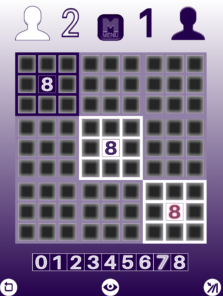
\includegraphics[scale=0.5]{img/tutorial_1.png}
\end{center}

\pagebreak
\begin{itemize}
    \item Players receive points equal to the number in the region where the number is placed. These points 
    are known as \textbf{Power}.
\end{itemize}
\begin{center}
    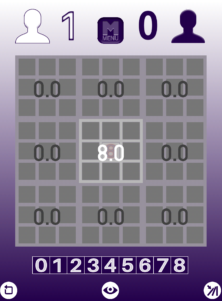
\includegraphics[scale=0.5]{img/tutorial_2.png}
\end{center}

\begin{itemize}
    \item If a number borders other regions, horizontally, vertically or diagonally, the player receives 
    1/2 points in those border regions.  These points are known as \textbf{Influence}.
\end{itemize}
\begin{center}
    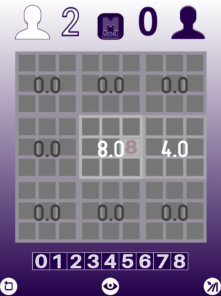
\includegraphics[scale=0.5]{img/tutorial_3.png}
\end{center}

\begin{itemize}
    \item Placement conforms to the rules of Sudoku, so a number may only be placed once in a region, row or 
    column. (Broken Sudoku will occur.)
    \item When all numbers that can be placed have been placed, the gameboard is resolved. \textbf{Resolution} 
    determines the outcome.
\end{itemize}

\pagebreak
\subsubsection{Resolution Phase}

\begin{itemize}
    \item Regions are resolved in order of the greatest disparity. These are the regions with greatest point 
    difference between players.
\end{itemize}
\begin{center}
    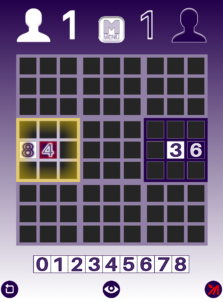
\includegraphics[scale=0.5]{img/tutorial_4.png}
\end{center}

\begin{itemize}
    \item When a region is resolved, it is awarded to the player with the most points in the region, known as the dominant player.
    \item All opposing numbers in that region defect, flipping to the dominant player. This player is now said to have control.
\end{itemize}
\begin{center}
    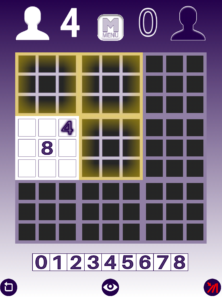
\includegraphics[scale=0.5]{img/tutorial_5.png}
\end{center}

\begin{itemize}
    \item If these numbers border other regions, they switch their \textbf{Influence} points. (This can shift the balance of power, 
    affecting the outcome of the game!)
\end{itemize}
\begin{center}
    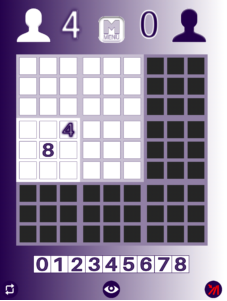
\includegraphics[scale=0.5]{img/tutorial_6.png}
\end{center}

\begin{itemize}
    \item When all regions that can be resolved, have been resolved, the player controlling the most regions wins.
    \item Strength of victory is measured by the ratio of controlled regions between players, such as 5/4, 4/5, 4/4, 9/0, 0/9,\ldots
\end{itemize}

\paragraph{}
The official rules can be consulted in the address: http://mbranegame.com/rules-of-m \cite{Rules}.

%%%%%%%%%%%%%%%%%%%%%%%%%%
\pagebreak
\section{Game Logic}

\subsection{Game state representation} 
Although the user can only see one board at a time, in a any phase of the game, there are actually three
boards represented in the game’s data structures. There’s a board predicate that represents the game \textbf{board} itself, a
list of 9 lists each representing a line of the board. This is the board used to print the state of the game. There’s 
also a \textbf{board\_blocks} predicate. This predicate is also a list of 9 lists, each one representing a 3 by 3 block of the 
board, this is used to facilitate calculations involving power in each block and influence in adjacent blocks caused 
by the placement of a number in the edge of a block. Finally we have a \textbf{board\_influence} list that stores the values of 
power (and spread influence) in each block of the board.  When a player adds a number to cell, all the boards are 
updated accordingly. The predicate used to declare a fresh board is \textit{start\_board(-Board)}, which unifies a variable to a list 
of containing the three boards mentioned above. In order to distinguish both players we determined that Player1 would place 
positive numbers on the board, and Player2 would place negative numbers. This eases the calculations and makes it possible 
to display to the user the which player has controll in each block of the board

\begin{center}
    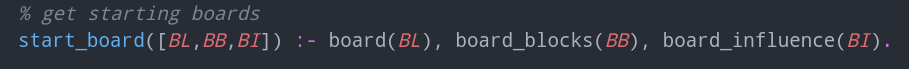
\includegraphics[scale=0.3]{img/board.png}
\end{center}




\subsection{Board viewing} 
Before each move, the board is displayed on the screen. To display the board we use the predicate \textit{display\_game(+Board, +Player1, +Player2)}. This predicate first displays the players' names and then uses \textit{display\_board(+Board)} to display the board itself. 
The board is displayed line by line with a series of dividers. Although for game logic the values of the board can be positive or negative, the board is printed with only positive numbers.
The power of all the blocks is also displayed using\textit{display\_power(+Power)}

\begin{center}
    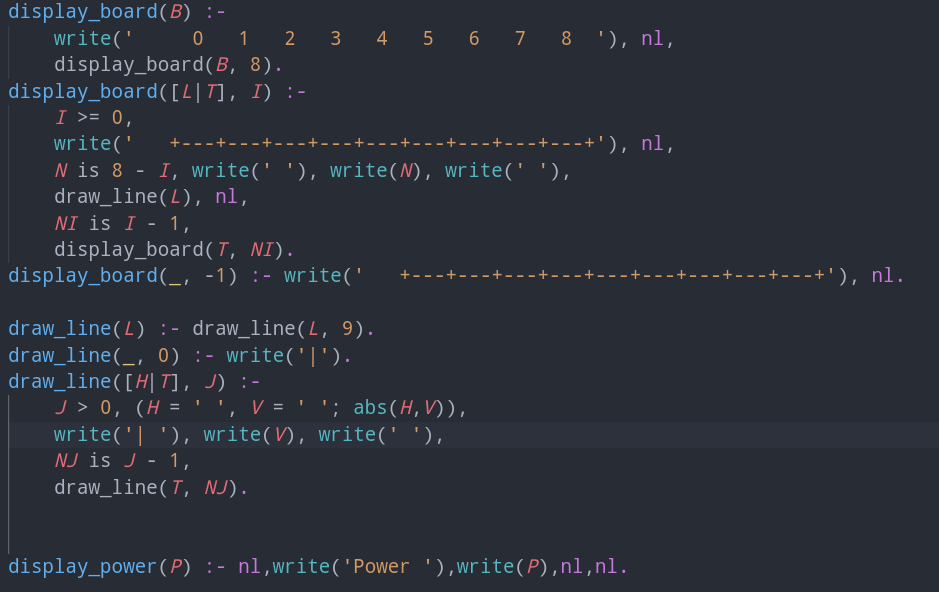
\includegraphics[scale=0.3]{img/display.png}
\end{center}


\subsection{List valid plays} 
As per requested, we developed a predicate that returns a list of all possible moves. This predicate is \textit{valid\_moves(+Board, -R)}. The first argument of the predicate is a list with the board of lines and board of blocks.
This predicate works by first finding a list of all empty cells with \textit{check\_all(+Board, -List),}. Then it tests all possible values in those cells with \textit{test\_all(+List, +Board, +Result)}.
\textit{R} is a list of all the possible moves which are also lists in the format \textit{[X,Y,Value]}.

\begin{center}
    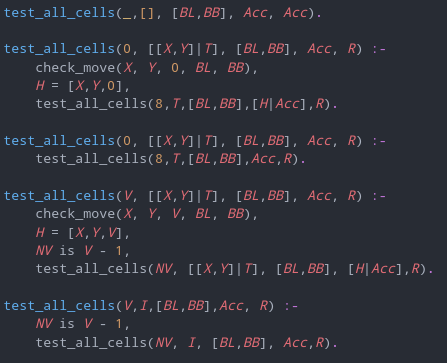
\includegraphics[scale=0.4]{img/test_all.png}
\end{center}



\subsection{Play execution} 
Each player can make a move per turn \textit{player\_turn(+Board, +Player, -NewBoard)}. In this turn predicate, the program asks the player what he wants to play with \textit{get\_move(-X, -Y, -V)} then the program tries that move with \textit{move(+Move, +Board, -NewBoard)}.
If the move is invalid the program repeats the previous action, otherwise, it returns a new board with the new piece.

\begin{center}
    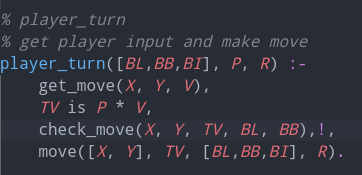
\includegraphics[scale=0.4]{img/player_turn.png}
\end{center}

\pagebreak
\subsection{Game finalization} 

\paragraph{}
The game is in the final state if no more numbers can be placed on the board, according to placing rule already 
mentioned. We know this using the \textit{valid\_moves(+Board, -R)}. If the Result list is empty, then no more valid
moves can be made, which means the game is in the final state. When this happens the \textit{game\_over(+Board, -Winner)}
predicate calculates the winner of the game.

\begin{center}
    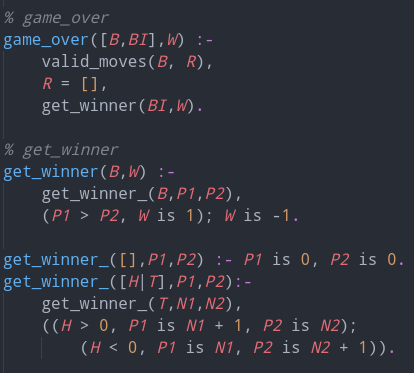
\includegraphics[scale=0.4]{img/game_over.png}
\end{center}

\subsection{Board evaluation}
\paragraph{}
The number placing rules are the ones of Sudoku, so the player can only place a number if that same number is not present
in either the column, row or 3x3 section of the square the player wants to place it. If these conditions are met, 
the number is able to be placed.

\paragraph{}
We evaluate if a play is possible using the \textit{check\_move(+X,+Y,+Value,+BL,+BB)}, it calculates if the move is possible using 
all the restrictions merntioned  above, if some of those restrictions are not met the predicate fails indicating the move can't be made.

\begin{center}
    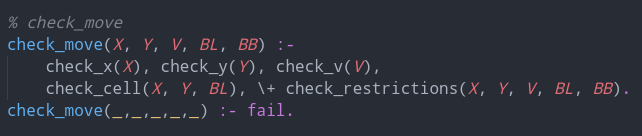
\includegraphics[scale=0.4]{img/check_move.png}
\end{center}

% TODO complete
\subsection{Plays of the computer} 
The computer plays only in an easy difficulty setting, this means that for each turn of the computer we get all the possible plays using 
the \textit{valid\_moves(+Board, -R)} predicate. Then using the \textit{random/3} predicate from the SicStus random library, we choose a random 
move and execute it. The predicate that makes the move move of the computer is \textit{bot\_turn(+Board,+Power,-Result)}.

\begin{center}
    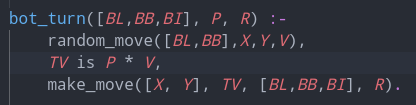
\includegraphics[scale=0.4]{img/bot_move.png}
\end{center}


%%%%%%%%%%%%%%%%%%%%%%%%%%
\pagebreak
\section{Conclusions}

\paragraph{}
Overall, the project was a really good way to practice the Prolog programming language, and
also see how it can be used to create a real application (in this case a game). In the 
begginning we really struggled to understand the implications of the language and how 
we could use it to build a game. The total change of paradigm from what we were used to 
was really tough and the learning curve was a really rough one. Our start was very slow 
and we took some time before we could start working at a decent pace.

\paragraph{}
We had a lot of trouble during the development of the project. Everything started on our first
approach to internally store and use the game board. Only when we were trying to make 
the game "playable" did we realize our approach was not the best one, as we were not finding a 
way to make the game play past the second round. This required an almost total refactoring of
the code which made us loose a lot of time. We ended up not having time to implement a more 
difficult game mode agains the computer using a little aritifitial inteligence which was 
something we were looking forward to do. Due to these time issues we also ended up not implementing
the final \textit{Resolution Phase}. We made this decision having in mind it whould not add much
 complexity to the project as it would only involve some calculations using already existing preicates.

\paragraph{}
In the end of the development of the project we actually were programming at a good rythm. So 
we find this was a positive experience, that helped us getting a better understanding 
of declarative programming languages and logic programming.


\clearpage
%\addcontentsline{toc}{section}{Bibliografia}
\renewcommand\refname{Apendix}
\bibliographystyle{apalike}
\bibliography{myrefs}

\newpage
\appendix
% \section{Nome do Anexo}
% Outros elementos úteis que não sejam essenciais ao relatório.

\end{document}
